\section{\scshape Sensors deployment}

\begin{frame}{Sensors deployment}
	\begin{itemize}
%		\item For making the estimation of the sensor disposition computational feasible, the 3D continuous space was populated with a given set of sensors that were looking at a given point (with the sensor roll either 0º or random)
		\item Several populations of sensors were added to each simulated world.
%		\begin{itemize}
%			\item The 3D sensor models will be hidden at rendering time to avoid occlusion of sensor data
%		\end{itemize}
		\item Each population is of a given sensor type and is deployed within a given region of interest.
%		\begin{itemize}
%			\item This allows to restrict the spatial distribution of the sensors, for example a given set of sensors should be in the walls or ceiling due to their weight, or they should be close to the target object given their limited depth measurements range
%		\end{itemize}
		\item Currently supported deployment configurations:
		\begin{itemize}
			\item Uniform along a line.
			\item Uniform within a 2D grid.
			\item Uniform or random deployment within a box.
			\item Uniform or random deployment within a cylinder.
		\end{itemize}
	\end{itemize}
\end{frame}


\begin{frame}{Sensors deployment for active perception}
	\begin{itemize}
		\item For the active perception environment, 450 sensors were deployed close to the target object, on the top, right and back side of the trolley.
%		\item This was done to simulate the closest range in which a dynamically moving sensor attached to a robotic arm could move (taking into consideration the human safety and the sensor minimum measurement distance, that was 0.2 meters).
	\end{itemize}
	\begin{figure}
		\centering
		\includegraphics[height=.63\textheight]{sensor-deployment/active-perception/gazebo-front}
		\includegraphics[height=.63\textheight]{sensor-deployment/active-perception/gazebo-top}
		\caption{Sensors deployment for the active perception environment (the CAD models of the sensors are hidden during the generation of the depth image).}
	\end{figure}
\end{frame}


\begin{frame}{Sensors deployment for single object bin picking}
	\begin{itemize}
%		\item For the single bin picking environments, given that the target object was inside the stacking box, the sensors were deployed close to the target object, but only on top of the trolley, on 3 layers (each with a different type of sensor).
		\item In the world with minimal occlusions it was deployed 100 sensors while in the world with significant occlusions it was deployed 300 sensors.
%		\begin{itemize}
%			\item The sensor density was increased given that the best views have tighter observation regions which could be missed with a sparse sensor deployment.
%		\end{itemize}
	\end{itemize}
	\begin{figure}
		\centering
		\includegraphics[height=.66\textheight]{sensor-deployment/bin-picking/gazebo-sensors}\hspace{3em}
		\includegraphics[height=.66\textheight]{sensor-deployment/bin-picking-with-occlusions/gazebo-sensors}
		\caption{Sensors deployment for the 2 bin picking environments that had a single target object.}
	\end{figure}
\end{frame}


\begin{frame}{Sensors deployment for multiple object bin picking}
	\begin{itemize}
		\item For the multiple bin picking environment, given that there were multiple target objects it was deployed 450 sensors across 7 populations:
		\begin{itemize}
			\item 5 populations simulating fixed sensors on the walls and ceiling.
			\item 2 populations above the trolley, simulating dynamic sensors attached to a robotic arm.
		\end{itemize}
	\end{itemize}
	\begin{figure}
		\centering
		\includegraphics[height=.55\textheight]{sensor-deployment/multiple-bin-picking-with-occlusions/gazebo-front}\hspace{2em}
		\includegraphics[height=.55\textheight]{sensor-deployment/multiple-bin-picking-with-occlusions/gazebo-top}
		\caption{Sensors deployment for the bin picking environment that had multiple target objects.}
	\end{figure}
\end{frame}
